%% 7. MICs

% Explain KNC
\begin{frame}{Many Integrated Core Architecture}
 
 \begin{block}{Background}
  \begin{itemize}
   \item Many-core architecture by Intel
   \item ``Just recompile'' existing OpenMP-enabled code
   \item Current: Knights Corner (Q4 2012)
   \item Upcoming: Knights Landing (Q1 2016)
  \end{itemize}
 \end{block}
 
 \begin{center}
  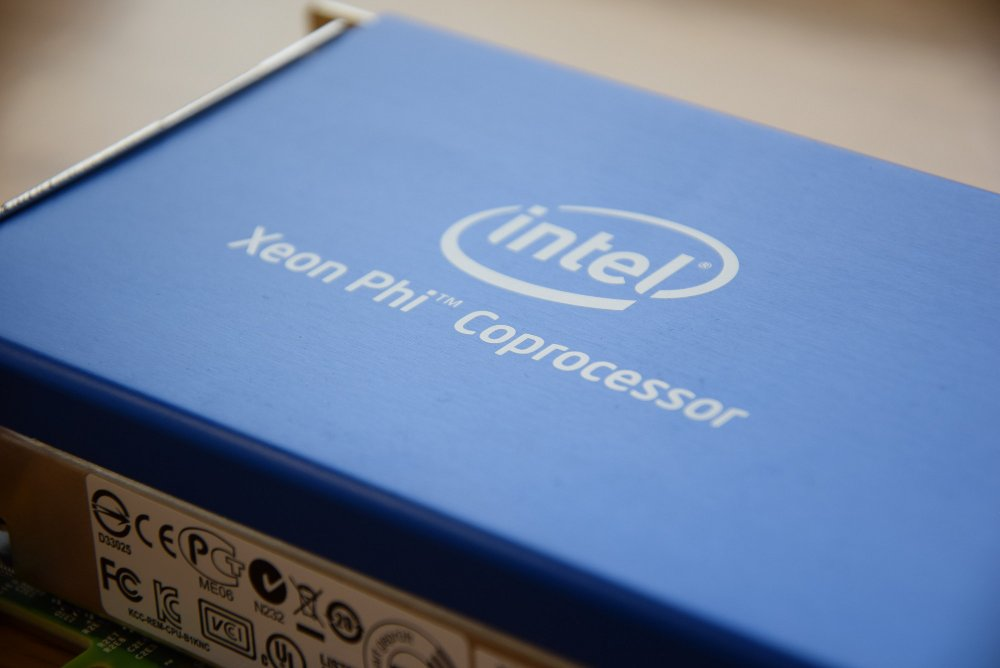
\includegraphics[width=0.5\textwidth]{figures/xeon-phi}
 \end{center}

\end{frame}

\begin{frame}{Many Integrated Core Architecture}
 
 \begin{block}{Knight Corner: Technical Details}
  \begin{itemize}
   \item High memory bandwidth: 320 GB/sec ideal, 160 GB/sec real
   \item High compute power: 1 TFLOP/sec (fp64)
   \item Fixed main memory: 8 or 16 GB
   \item Custom operating system on board
  \end{itemize}
 \end{block}
 
 \vspace*{-0.5cm}
 \begin{center}
  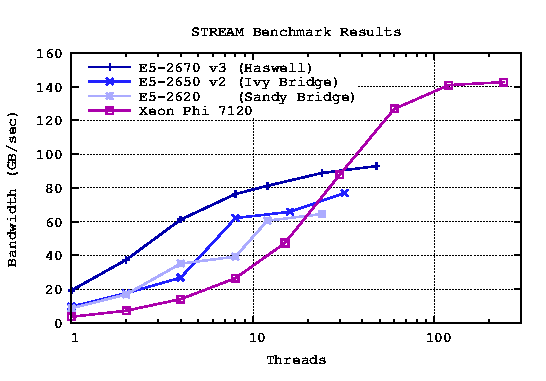
\includegraphics[width=0.7\textwidth]{figures/stream}
 \end{center}

\end{frame}


\begin{frame}{Many Integrated Core Architecture}
 
 \begin{block}{Knights Corner: Problems}
  \begin{itemize}
   \item Very low single-thread performance
   \item ``Just recompile'' almost never enough
   \item PCI-Express communication slower than for GPUs
   \item Even Intel now recommends Haswell-Xeons over Knights Corner
  \end{itemize}
 \end{block}
 
 %\pause
 \begin{center}
  
\includegraphics[width=0.65\textwidth]{figures/xkcd-someone-wrong} \\
  {\scriptsize http://xkcd.com/386/}
 \end{center}

\end{frame}


% Explain new stuff for KNL

\begin{frame}{Many Integrated Core Architecture}
 
 \begin{block}{KNL: Compute}
  \begin{itemize}
   \item 72 cores
   \item Energy-efficient IA cores
   \item 3x single-thread performance vs. KNC
   \item Binary compatibility with Xeon line
   \item 3+ TFLOPS in double precision
  \end{itemize}
 \end{block}

 \begin{block}{KNL: On-Package Memory}
  \begin{itemize}
   \item 16 GB
   \item 5x bandwidth vs. DDR4
   \item 5x power efficiency vs. DDR4
  \end{itemize}
 \end{block}
 
\end{frame}


\begin{frame}{Many Integrated Core Architecture}
 
 \begin{block}{KNL Schematic}
  \begin{itemize}
   \item 36 tiles interconnected by 2D mesh
   \item Each tile: 2 cores, 2 vector units per core, 1 MB L2 cache
  \end{itemize}
 \end{block}
 
 \begin{center}
  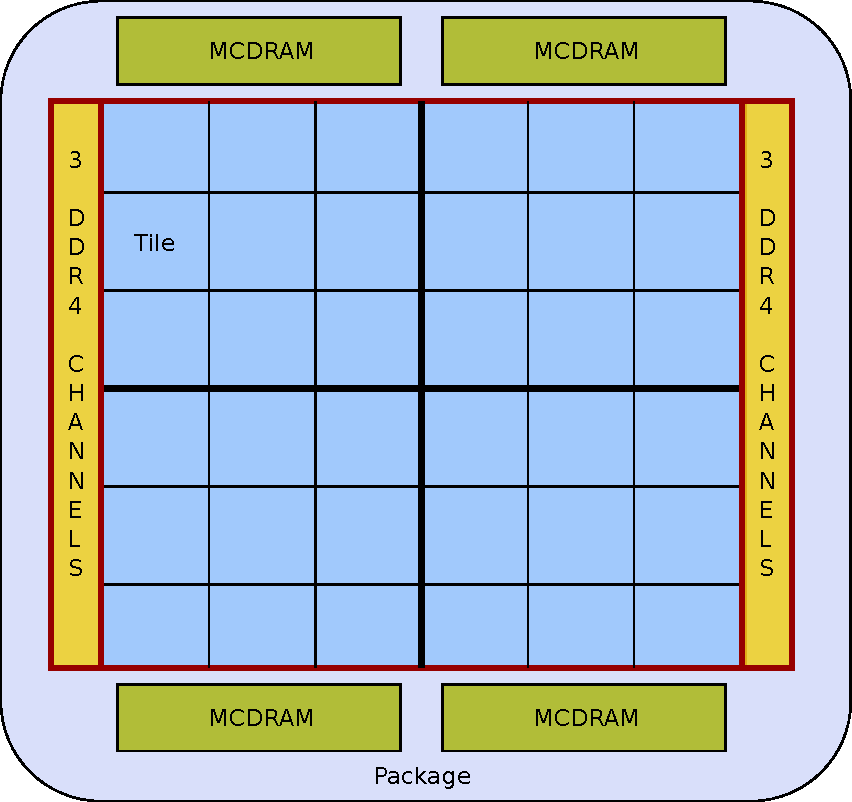
\includegraphics[width=0.5\textwidth]{figures/knl-schematic} \\
 \end{center}
\end{frame}

\begin{frame}{Many Integrated Core Architecture}
 
 \begin{block}{HBM: Cache Mode}
  \begin{itemize}
   \item No code changes necessary
   \item Cache misses expensive
  \end{itemize}
 \end{block}

 \begin{block}{HBM: Flat Mode}
  \begin{itemize}
   \item MCDRAM mapped to physical address space
   \item Exposed as NUMA node
   \item Accessed through memkind library or numactl
  \end{itemize}
 \end{block}

 \begin{block}{HBM: Hybrid Mode}
  \begin{itemize}
   \item Combination of the above two
   \item Get the best and worst of two worlds
  \end{itemize}
 \end{block}

\end{frame}

